\documentclass[12pt]{article}
\usepackage{amsfonts}
\usepackage{fancyhdr}
\usepackage[a4paper, top=2.5cm, bottom=2.5cm, left=2.2cm, right=2.2cm]{geometry}
\usepackage{times}
\usepackage{amsmath}
\usepackage{changepage}
\usepackage{amssymb}
\usepackage{graphicx}%
\setcounter{MaxMatrixCols}{30}
\newtheorem{theorem}{Theorem}
\newtheorem{acknowledgement}[theorem]{Acknowledgement}
\newtheorem{algorithm}[theorem]{Algorithm}
\newtheorem{axiom}{Axiom}
\newtheorem{case}[theorem]{Case}
\newtheorem{claim}[theorem]{Claim}
\newtheorem{conclusion}[theorem]{Conclusion}
\newtheorem{condition}[theorem]{Condition}
\newtheorem{conjecture}[theorem]{Conjecture}
\newtheorem{corollary}[theorem]{Corollary}
\newtheorem{criterion}[theorem]{Criterion}
\newtheorem{definition}[theorem]{Definition}
\newtheorem{example}[theorem]{Example}
\newtheorem{exercise}[theorem]{Exercise}
\newtheorem{lemma}[theorem]{Lemma}
\newtheorem{notation}[theorem]{Notation}
\newtheorem{problem}[theorem]{Problem}
\newtheorem{proposition}[theorem]{Proposition}
\newtheorem{remark}[theorem]{Remark}
\newtheorem{solution}[theorem]{Solution}
\newtheorem{summary}[theorem]{Summary}
\usepackage{enumitem}
\usepackage[utf8]{inputenc}
\newenvironment{proof}[1][Proof]{\textbf{#1.} }{\ \rule{0.5em}{0.5em}}
\usepackage{tikz}
\usepackage{graphicx}
\usepackage{wrapfig}
\usepackage{float}
\usepackage{datetime}
\newdateformat{specialdate}{\twodigit{\THEDAY}.\twodigit{\THEMONTH}.\THEYEAR}


\newcommand{\Q}{\mathbb{Q}}
\newcommand{\R}{\mathbb{R}}
\newcommand{\C}{\mathbb{C}}
\newcommand{\Z}{\mathbb{Z}}

\begin{document}
	
	\title{1. Übung}
	\author{Timo Bergerbusch 344408 \& Marc Burani-Mc 1337-GG}
	\date{\specialdate\today}
	\maketitle
	
	
	\section{Aufgabe 1}
	\begin{enumerate}[label=(\alph*)]
		\item \begin{enumerate}[label=(\roman*)] 
				\item Planen von Postbotenrouten
				\item Planen der Standorte von Verteil-Zentren
				\item Berechnung der Optimalen Transportmengen Aufteilung in der Logistik
				\item Zuschneiden von Stoffen/Metallen/Kunststoffen/... für möglichst geringen Verschnitt
				\item Planen von Belegungsplänen von Räumen und Personal
			\end{enumerate}
		\item Eine Simulation ist eine reine Beispielausführung verschiedener Handlungsausführungen. Diese bietet keine Entscheidung oder Garantie sondern dient nur als Visualisierung. \newline
		Eine Optimierung hingegen ist das Ableiten einer (optimalen) Entscheidung für verschiedene Alternativen auf Grund von Nutzenfunktionen. Optimierung kann Simulationen nutzen um Situationen zu prüfen.
		\item Ein Problem ist ein allgemeiner Begriff für ein theoretische Fragestellung. Eine Instanz hingegen ist eine konkrete Ausprägung eines Problems. \newline
		\textbf{Beispiel}: Das Traveling-Salesman-Problem ist ein Problem und eine TSP-Reise über die Städte Berlin, München, Stuttgart und Köln ist eine Instanz des allgemeinen Problems.
		\item Eine \textit{optimale} Lösung $L$, mit $\mathbb{L}$ der Raum aller zulässigen Lösungen und $f$ die Nutzenfunktion, muss folgende Eigenschaften erfüllen:
			\begin{itemize}
				\item $L \in \mathbb{L}$
				\item $\forall L^\prime \in \mathbb{L}: f(L^\prime) \le f(L)$
			\end{itemize}
		\item Indem man sich eine Untere Schrank bei Minimierungsproblemen und eine Obere Schranke bei Maximierungsproblemen herleitet und den Abstand dieser zur aktuellen Lösung misst. Bei einem "geringen" Abstand ist eine weitere Optimierung schwer erreichbar und weniger lohnend als bei einer "großen" Abweichung. Allerdings sind "gering" und "groß" in jeder Situation relativ zu sehen.
	\end{enumerate}

	\section{Aufgabe 2}
	\begin{enumerate}[label=(\alph*)]
		\item 
		\item \textbf{symetrisches TSP}: Der Graph hat ungerichtete Kanten. Somit dauert eine Reise von Stadt A zu Stadt B genauso lange wie eine Reise von Stadt B zu Stadt A.\newline
		\textbf{asymetrisches TSP}: Der Graph hat gerichtete Kanten. Somit ist es möglich, dass eine Reise von Stadt A zu Stadt B die Dauer $d$ hat und die Reise von Stadt B zu Stadt A die Dauer $d^\prime$ mit $d \neq d^\prime$\newline
		In der gegebenen Probleminstanz handelt es sich um eine symmetrische Matrix.
		\item 
		\item
		\item
	\end{enumerate}

	\section{Aufgabe 3}
	\begin{enumerate}[label=(\alph*)]
		\item Ein \textit{Algorithmus} ist eine deterministische imperative Abfolge von verschiedenen Operationen zur Lösung eines Problems durch eine endliche, teils rekursive oder sich wiederholende Folge von Anweisungen.
		\item Ein Algorithmus ist: \begin{itemize}
				\setlength{\itemindent}{2in}
				\item[eindeutig:] Reihenfolge der Schritte ist deterministisch
				\item[allgemein:] es wird ein Problem und nicht eine Probleminstanzen gelöst
				\item[ausführbar:] ein Prozessor muss die Einzelschritte abarbeiten können
				\item[endlich:] seine Beschreibung ist endlich Lang. (Lässt sich als Turingmaschine aufschreiben)			
			\end{itemize}
		\item Ein Problem $P$ lässt sich auf ein anderes Problem $P^\prime$ \textit{polynomiell Reduzieren}, wenn es polynomiell berechenbare Funktionen $f$ und $g$ gibt sodass folgendes gilt:
			\begin{itemize}
				\item $f$ projiziert Instanzen von $P$ auf Instanzen von $P^\prime$
				\item $g$ projiziert Lösungen von $P^\prime$ auf Lösungen von $P$
			\end{itemize}
		\item 
		Für ein Programm $P$:
		\textbf{NP-Schwer}: $\forall P^\prime\in NP: P^\prime\text{ ist poly. Red. auf }P$ \newline
		\textbf{NP-Vollständig}: $P\in \mathbb{NP}$ und $P$ ist $NP$-Schwer \newline
		Jedes NP-Vollständige Problem ist NP-Schwer allerdings gibt es Problem, welche zwar NP-Schwer sind jedoch nicht zwingend in NP liegen
		\item Keine.
		\item \begin{enumerate}
			\item Allgemeinheit
			\item Effizienz (Zeit \& Speicher)
			\item Optimalität
		\end{enumerate}
	\end{enumerate}

	\section{Aufgabe 4}
	
	\begin{enumerate}[label=(\alph*)]
		\item Pfad:
			\begin{figure}[H]
				\centering
				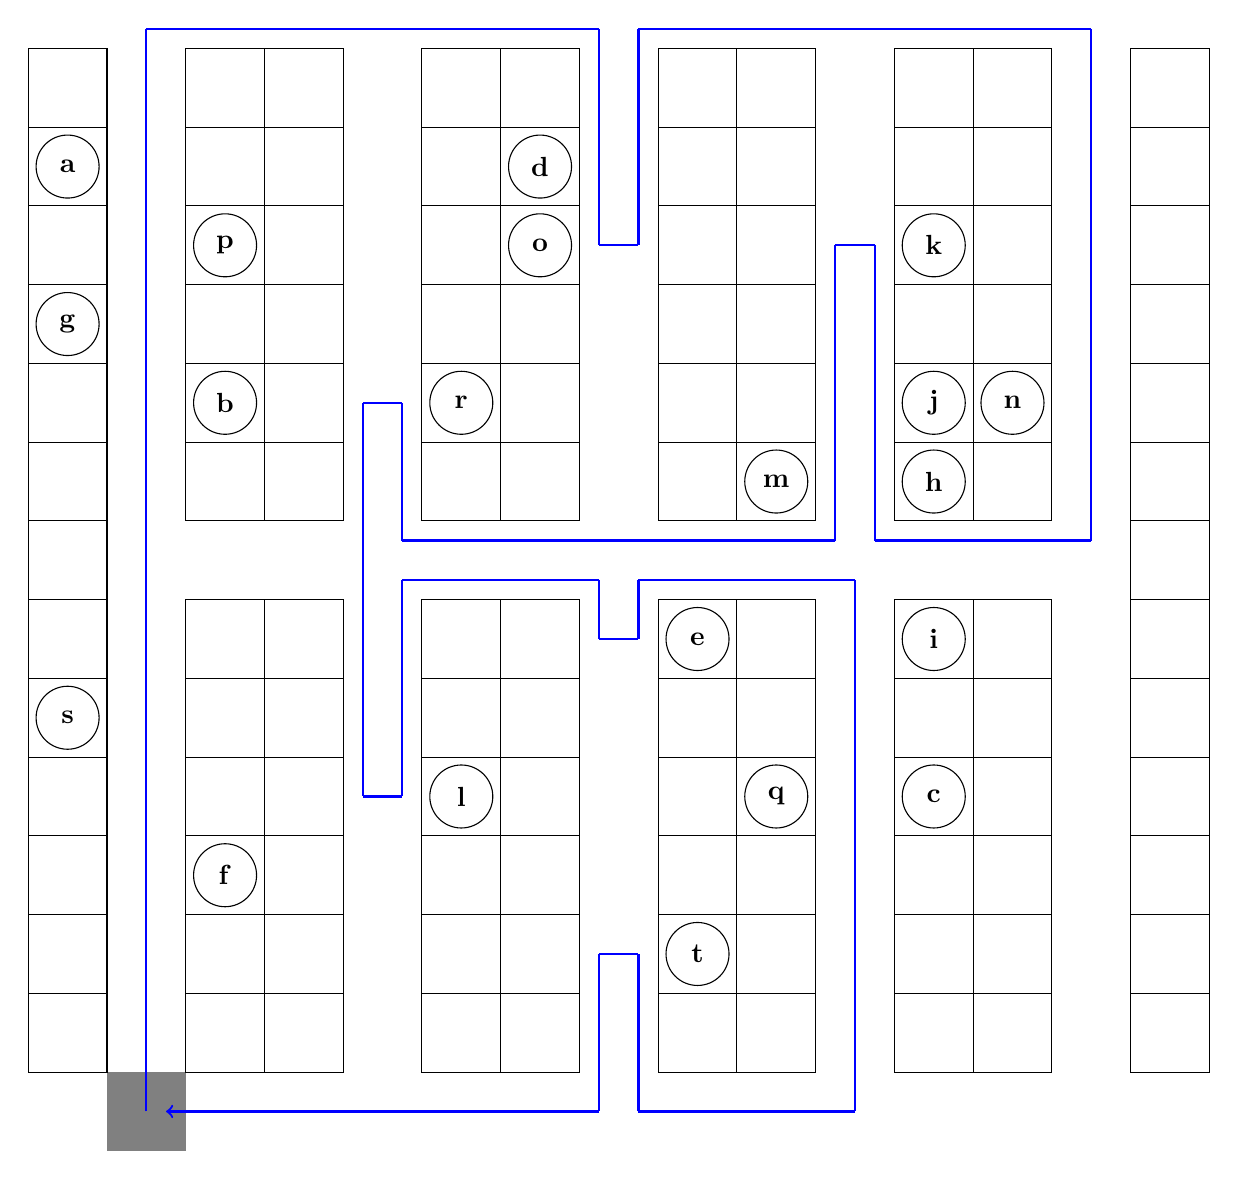
\begin{tikzpicture}		
				
					\fill[white!50!black] (1,0) rectangle (2,1);	
						
					\foreach \x in {1,...,13}
						\draw (0,\x) rectangle (1,\x+1);
						
					\foreach \y in {2,3,5,6,8,9,11,12}
						\foreach \x in {1,...,6,8,9,10,11,12,13}
							\draw (\y,\x) rectangle (\y+1,\x+1);
							
					\foreach \x in {1,...,13}
					\draw (14,\x) rectangle (15,\x+1);
					
					\draw (.5,5.5) circle (.4cm) node {\textbf{s}};
					\draw (.5,10.5) circle (.4cm) node {\textbf{g}};
					\draw (.5,12.5) circle (.4cm) node {\textbf{a}};
					
					\draw (2.5,3.5) circle (.4cm) node {\textbf{f}};
					\draw (2.5,9.5) circle (.4cm) node {\textbf{b}};
					\draw (2.5,11.5) circle (.4cm) node {\textbf{p}};
					
					\draw (5.5,4.5) circle (.4cm) node {\textbf{l}};
					\draw (5.5,9.5) circle (.4cm) node {\textbf{r}};
					
					\draw (6.5,11.5) circle (.4cm) node {\textbf{o}};
					\draw (6.5,12.5) circle (.4cm) node {\textbf{d}};
					
					\draw (8.5,2.5) circle (.4cm) node {\textbf{t}};
					\draw (8.5,6.5) circle (.4cm) node {\textbf{e}};
					
					\draw (9.5,4.5) circle (.4cm) node {\textbf{q}};
					\draw (9.5,8.5) circle (.4cm) node {\textbf{m}};
					
					\draw (11.5,4.5) circle (.4cm) node {\textbf{c}};
					\draw (11.5,6.5) circle (.4cm) node {\textbf{i}};
					\draw (11.5,8.5) circle (.4cm) node {\textbf{h}};
					\draw (11.5,9.5) circle (.4cm) node {\textbf{j}};
					\draw (11.5,11.5) circle (.4cm) node {\textbf{k}};
					
					\draw (12.5,9.5) circle (.4cm) node {\textbf{n}};
					
					\draw[blue,thick] (1.5,0.5) -- (1.5,14.25);
					\draw[blue,thick] (1.5,14.25) -- (7.25,14.25);
					
					\draw[blue,thick] (7.25,14.25) -- (7.25,11.5);
					\draw[blue,thick] (7.25,11.5) -- (7.75,11.5);
					\draw[blue,thick] (7.75,11.5) -- (7.75,14.25);
					
					\draw[blue,thick] (7.75,14.25) -- (13.5,14.25);
					
					\draw[blue,thick] (13.5,14.25) -- (13.5,7.75);
					
					\draw[blue,thick] (13.5,7.75) -- (10.75,7.75);
					\draw[blue,thick] (10.75,7.75) -- (10.75,11.5);
					\draw[blue,thick] (10.75,11.5) -- (10.25,11.5);	
					\draw[blue,thick] (10.25,11.5) -- (10.25,7.75);	
					
					\draw[blue,thick] (10.25,7.75) -- (4.75,7.75);
					\draw[blue,thick] (4.75,7.75) -- (4.75,9.5);
					\draw[blue,thick] (4.75,9.5) -- (4.25,9.5);
					\draw[blue,thick] (4.25,9.5) -- (4.25,4.5);
					\draw[blue,thick] (4.25,4.5) -- (4.75,4.5);
					\draw[blue,thick] (4.75,4.5) -- (4.75,7.25);
					
					\draw[blue,thick] (4.75,7.25) -- (7.25,7.25);
					\draw[blue,thick] (7.25,7.25) -- (7.25,6.5);
					\draw[blue,thick] (7.25,6.5) -- (7.75,6.5);
					\draw[blue,thick] (7.75,6.5) -- (7.75,7.25);
					
					\draw[blue,thick] (7.75,7.25) -- (10.5, 7.25);
					\draw[blue,thick] (10.5,7.25) -- (10.5,0.5); 
					
					\draw[blue,thick] (10.5,0.5) -- (7.75,0.5);
					\draw[blue,thick] (7.75,0.5) -- (7.75,2.5);
					\draw[blue,thick] (7.75,2.5) -- (7.25,2.5);
					\draw[blue,thick] (7.25,2.5) -- (7.25,0.5);
					
					\draw[blue,thick,->] (7.25,0.5) -- (1.75,0.5);
				\end{tikzpicture}
			\end{figure}
		\item ???
		\item \textbf{Nein}. Gegenbeispiel:\\
			\begin{figure}[H]
				\centering
				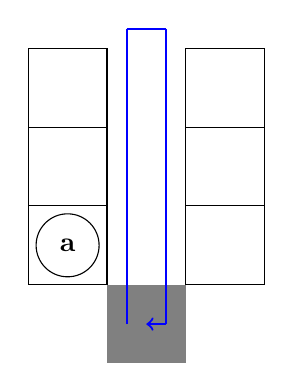
\begin{tikzpicture}
				
					\foreach \x in {1,2,3}
						\draw (0,\x) rectangle (1,\x+1);
						
					\foreach \x in {1,2,3}
						\draw (2,\x) rectangle (3,\x+1);
					
					\draw (0.5,1.5) circle (0.4cm) node {\textbf{a}};
					
					\fill[white!50!black] (1,0) rectangle (2,1);
					
					\draw[blue, thick] (1.25,0.5) -- (1.25,4.25);
					\draw[blue, thick] (1.25,4.25) -- (1.75,4.25);
					\draw[blue, thick] (1.75,4.25) -- (1.75,0.5);
					\draw[blue, thick, ->] (1.75,0.5) -- (1.5,0.5);
				\end{tikzpicture}
			\end{figure}
		Hier würde die \textit{Largest Gap} Heuristik hingehen und bis an das Ende der Reihe gehen, was allerdings nicht nötig ist. Somit ist es nicht exakt/optimal.
		\item Die \textit{Largest Gap} Heuristik liegt in ...
	\end{enumerate}

	\section{Aufgabe 5}
	\begin{enumerate}[label=(\alph*)]
		\item 
		\item
		\item
		\item
		\item
		\item
	\end{enumerate}
\end{document}


















